\documentclass[tikz, border=1mm]{standalone}
\usepackage{tikz} 
\usetikzlibrary{arrows.meta}
\usepackage{pgfplots}

\begin{document}

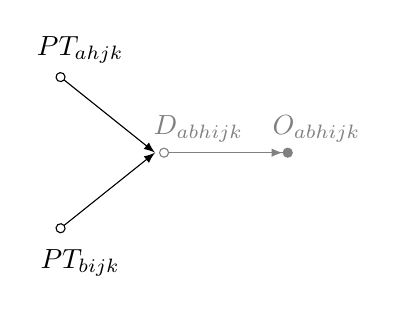
\begin{tikzpicture}

    % outcome
    \node[gray] at (3.5,1) {$O_{abhijk}$}; %[gray]

    % difference
    \node[gray] at (2,1) {$D_{abhijk}$}; %[gray]
    \draw[{Circle[open]}-{latex}{Circle},gray](1.5,0.7) to (3.2,0.7); %,gray

    %%%%%%%%%%%%%%%%%%%%%%%%%%%%%%%%%%%%%%%%%%%%%%%%%%%%%%%%%
    
    % "perceived" discriminal process for sub-unit
    \node at (0.5,2) {$PT_{ahjk}$}; %[gray]
    \draw[{Circle[open]}-{latex}](0.2,1.7) to (1.45,0.7); %,gray

    % "perceived" discriminal process for sub-unit
    \node at (0.5,-0.7) {$PT_{bijk}$}; %[gray]
    \draw[{Circle[open]}-{latex}](0.2,-0.3) to (1.45,0.7); %,gray  

    %%%%%%%%%%%%%%%%%%%%%%%%%%%%%%%%%%%%%%%%%%%%%%%%%%%%%%%%%

    %% "true" discriminal process for sub-unit
    %\node at (-1.5,2) {$T_{ah}$}; %[gray]
    %\draw[{Circle[open]}-{latex}](-1.7,1.68) to (0.15,1.68); %,gray 
    
    % judges' biases
    %\node at (-1.7,1.05) {$B_{kj}$}; %[gray]
    %\draw[{Circle[open]}-{latex}](-1.7,0.7) to (0.15,1.62); %,gray
    %\draw[-{latex}](-1.6,0.7) to (0.15,-0.22); %,gray 

    % "true" discriminal process for sub-unit
    %\node at (-1.5,0) {$T_{bi}$}; %[gray]
    %\draw[{Circle[open]}-{latex}](-1.7,-0.28) to (0.15,-0.28); %,gray     
    
\end{tikzpicture}

\end{document}
